\chapter[CredsRead]{CredsRead\raisebox{.3\baselineskip}{\normalsize\footnotemark}}
\footnotetext{\url{https://github.com/oliviercailloux/creds-read}}

CredsRead, pour Credentials Read, gère comme son nom l'indique la lecture des identifiants d'un utilisateur. Celle-ci s'effectue de trois manières, comme pour l'authenfication dans Plaquette-MIDO, les propriétés du système, les variables d'environnement et un fichier texte.

\section{Diagramme de classe}
Le diagramme de classe permet d'avoir une idée précise du code que l'on veut écrire. Papyrus est un outil permettant de réaliser ce genre de diagramme. Son interface intuitive facilite la rédaction d'un diagramme UML(le langage standard des diagrammes de classe) lisible et rigoureux. 

\begin{figure}[!h]
    \begin{center}
    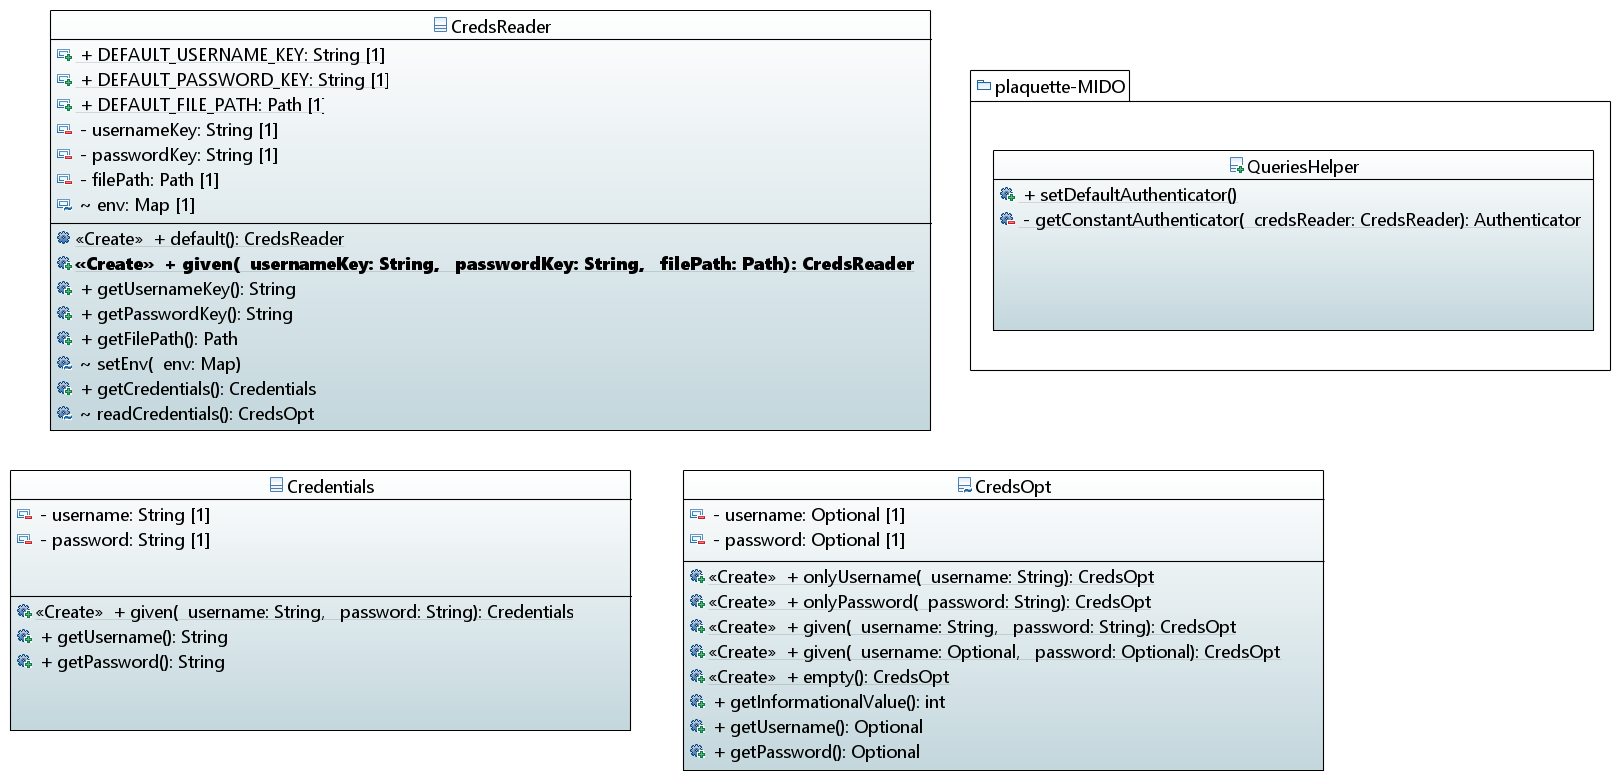
\includegraphics[width=\textwidth]{assets/doc.png}
    \end{center}
    \caption{Diagramme de classe du projet CredsRead}
\end{figure}


Le projet est composé de trois classes représentées par les différents blocs. Chaque bloc est constitué de son nom, suivi d'une partie avec l'ensemble des variables de la classe, et d'une partie avec l'ensemble des méthodes de la classe. Les éléments soulignés sont des statiques. Le symbole $+$ précédant les éléments indique qu'ils sont publics, le $-$ privés, le $\sim$ de visibilité package\footnote{En dehors du projet, ces éléments ne sont pas accessibles.}. Les méthodes sont présentées de cette façon \texttt{nomDeMethode(paramètres d'entrée): objet de sortie}. Le préfixe \texttt{Create} indique que ce sont des méthodes de construction. Il y a également un sous-dossier de plaquette-MIDO contenant la classe \texttt{QueriesHelper}. Celle-ci ne contient plus que deux méthodes spécifiques à la connexion à l'API de Dauphine.


\section{Les différentes classes}

\subsection{\texttt{CredsOpt}}
Cette classe remplace la classe \texttt{Authentication}, elle crée un objet contenant les identifiants de l'utlisateur, le nom d'utilisateur et le mot de passe, avec le type \texttt{Optional}. Celle-ci permet d'instancer également l'abscence d'information avec un \texttt{Optional} vide. Une distinction est ainsi faite entre un \texttt{Optional} vide (absence d'information) et un \texttt{String} vide : \texttt{""}. Ce dernier représente un nom d'utilisateur ou un mot de passe vide. La méthode \texttt{getInformationValue()} renvoie le nombre d'informations présentes (différente d'un \texttt{Optional} vide) dans l'objet \texttt{CredsOpt} (0, 1 ou 2).

Cette classe est de visibilité package, elle n'est utilisée que par les autres classes du package et n'est pas accessible publiquement.

\subsection{\texttt{Credentials}}
Cette classe crée également un objet contenant les identifiants, le nom d'utilisateur et le mot de passe. Ceux-ci sont cette fois de type \texttt{String}. Par rapport à \texttt{CredsOpt}, cette classe, ne permet pas d'instancer l'abscence d'information. 

Cette classe est publique, elle peut être utilisée en dehors du package par les utilisateurs.

\subsection{\texttt{CredsReader}}
\texttt{CredsReader} est la classe principale du projet. Elle est instancée par trois variables : une clé pour le nom d'utilisateur \texttt{usernameKey}, une clé pour le mot de passe \texttt{passwordKey} et un chemin vers un fichier \texttt{filePath}. Les deux clés sont utilisées pour lire les propriétés du système et les variables d'environnement. Le chemin correspond au fichier texte contenant les informations d'identification.

L'utilisateur peut créer un objet \texttt{CredsReader} en utilisant ses propres noms pour les variables d'instances. Il peut aussi utiliser les valeurs par défaut de la classe : \texttt{API\_username}, \texttt{API\_password}, \texttt{API\_login.txt}. Ces derniers sont ceux utlisés dans plaquette-MIDO.

\subsubsection{\texttt{readCredentials()}}
Voir annexe~\ref{sec:readCredentials()}.

\texttt{readCredentials()} est la méthode la plus importante de la classe. Elle est de visibilité package, elle n'est pas accessible aux utilisateurs. Elle renvoie un \texttt{CredsOpt}.

Elle permet de lire les informations d'identification : nom d'utilisateur et mot de passe. Pour chaque information, on distingue l'information manquante et la \texttt{String} vide. La méthode prend en compte les sources possibles suivantes :

\begin{enumerate}
    \item l.3 à 11 : Propriétés du système. Chaque propriété peut être définie, y compris pour la chaîne vide, ou non définie. Une information est considérée comme manquante (dans la source des propriétés) si la propriété correspondante n'est pas définie.
    \item l.13 à 21 : Variables d'environnement. Chaque variable peut être définie, y compris par une chaîne vide, ou non définie. Une information est considérée comme manquante (dans la source des variables d'environnement) si la variable d'environnement correspondante n'est pas définie.
    \item l.23 à 55: Fichier texte. Les deux informations sont considérées comme manquantes (de la source des fichiers) si le fichier n'existe pas. Si le fichier existe, aucune information n'est considérée comme manquante. La première ligne du fichier donne le nom d'utilisateur, la seconde le mot de passe. Si le fichier n'a qu'une seule ligne, le mot de passe (provenant de la source des fichiers) est mis à vide. Si le fichier est vide, les deux informations (provenant de la source des fichiers) sont fixées à la \texttt{String} vide. Les lignes vides ne sont pas prises en compte du tout. Si le fichier ne contient pas de ligne vide après la deuxième ligne, une exception est lancée.
\end{enumerate}
l.51 à 61 : La méthode a une logique de meilleure information de connexion. La source utilisée pour renvoyer un \texttt{CredsOpt} contenant les informations est celle qui a la valeur informationnelle la plus élevée, telle que déterminée par \texttt{CredsOpt.getInformationalValue()} (ce qui signifie que les sources sont classées par ordre croissant du nombre d'informations manquantes), et, dans le cas d'un fichier ex-\ae quo, l'ordre de priorité, tel que présenté ci-dessus, détermine quelle source est choisie.

\subsubsection{\texttt{getCredentials()}}
Voir annexe~\ref{sec:getCredentials()}

\texttt{getCredentials()} est la classe publique renvoyant un \texttt{Credentials}. Elle utlise la méthode \texttt{readCredentials()} pour récupérer la meilleure information d'identification (logique de priorité). Elle lance une exception si une (ou les deux) information manque.

\section{Intégration à plaquette-MIDO}

Le projet CredsRead a d'abord été édité dans le projet Plaquette-MIDO. Il a ensuite été séparé du projet initial. Il fallait donc l'intégrer. Pour cela, le projet CredsRead est publié sur Maven Central. Le projet peut alors être intégré à plaquette-MIDO en l'ajoutant dans le \texttt{pom.xml} et de cette façon être utilisé dans la classe \texttt{QueriesHelper} de plaquette-MIDO.

\begin{figure}[!ht]
    \lstinputlisting[language=Java, firstline=9, lastline=28]{assets/QueriesHelper.java}
    \caption*{La classe \texttt{QueriesHelper}, utilisant le projet CredsRead pour plaquette-MIDO.}
\end{figure}